\chapter{Evaluation}\label{ch:Evaluation}

In diesem Kapitel werden die Ergebnisse der einzelnen Phasen der Thesis beschrieben. Nach jeder Phase wurden Simulationen mit der Implementierung gestartet und verschiedene Informationen aufgezeichnet. Der Hauptgrund hierfür ist, dass durch die Ergebnisse zum einen ein allgemeines Gefühl für den Schwarm gegeben werden kann und wie er einzustellen ist. Zum anderen liefern die Beobachtungen wichtige Informationen für die späteren Phasen der Konzeption.
In diesem Kaputel werden nicht alle Statistiken vorgestellt, sondern nur die, die als interessant empfunden wurden.

\section{Generelles zur Evaluation}

Da die Roboter des Schwarms einen gewissen freien Willen haben, der entscheidet wo sie hinfahren, und dieser schlicht Zufall ist, werden die Simulationen mit ihren Parametern immer mehrmals durchgeführt. Um Ausreißer in der Auswertung auszumerzen, wurde ebenfalls nicht mit einem normalen Durchschnitt gerechnet, sondern mit einem Durchschnitt über die mittleren Ergebnisse.

Da die Simulationen mit über 5 Parametern weit mehr als 100 verschiedene Einstellungen zulassen, konnte nicht jede Konfiguration getestet werden. Stattdessen wurden die Einstellungen für die Simulationen durch Überlegung und den Ergebnissen der vorangegangenen Simulationen ausgewählt um die Anzahl im Bereich des zeitlich machbaren zu halten.

\section{Nachbau des Schwarms nach Craig Reynolds}

\begin{wrapfigure}{r}{\pictureWidth}
	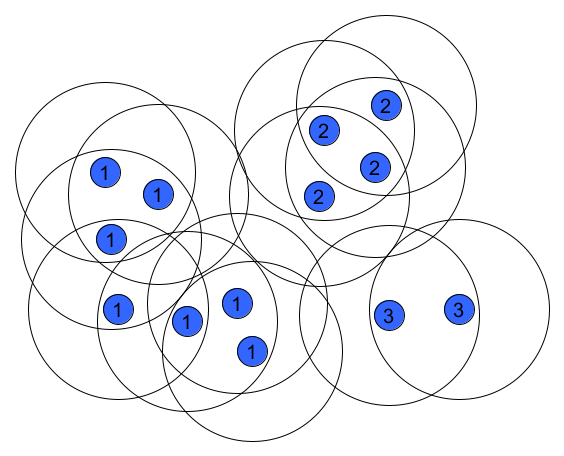
\includegraphics[width=\pictureWidth,keepaspectratio]{graphics/SchwarmEinordnung.png}
	\caption{Einordnung der Roboter in Schwärme}
	\label{pic:SchwarmEinordnung}
\end{wrapfigure}

Nachdem die Implementierung des Schwarms abgeschlossen ist, galt es diese zu testen und Statistiken zu erheben. Dazu wurde die Simulation mit verschiedenen Parametern gestartet und 25 Roboter zufällig in der Simulation verteilt. Die Simulationen wurden für 1 Stunde laufen gelassen und in 10s-Abständen gemessen, wie viele Schwärme sich gebildet haben.
Ein Schwarm war hierbei eine zusammenhängende Kette von Robotern, die nicht weiter als ihre lokale Reichweite voneinander entfernt sind. Das bedeutet, dass alle Roboter innerhalb eines Schwarm die anderen beeinflussen. Teilweise mag dies direkt geschehen sein, wenn sie innerhalb der lokalen Reichweite waren. Aber auch indirekte Beeinflussung ist es möglich, indem Roboter beeinflusst wurden, durch Roboter die von anderen beeinflusst wurden. \autoref{pic:SchwarmEinordnung} zeigt ein Beispiel mit 3 Schwärmen. Die Roboter sind als blaue Kreise eingezeichnet, ihre jeweilige lokale Reichweite als schwarzer Kreis drum herum. Eine Zahl im inneren zeigt die Zugehörigkeit zum jeweiligen Schwarm.

Da das Verhalten der Roboter, aufgrund ihres freien Willens und der zufälligen Platzierung in der Simulation, starken Schwankungen ausgesetzt ist, wurden immer 10 Simulationen gestartet und aus den mittleren 6 Werten ein Durchschnitt gebildet. Dadurch wurden Ausreißer eliminiert und die Statistiken können sinnvolle Mittelwerte zeigen. Der Rand der Simulation wurde als Hinderniss gewertet, was bedeutet, dass die Roboter nicht stumpf weiter gefahren sind nachdem dieser erreicht wurde, sondern sie versucht haben diesem auszuweichen.

\subsection*{Statistik: Freier Wille}\label{subsubsec:StatistikFreierWille}

\begin{table}[h]
	\caption{Eigenschaften des Schwarms}
	\begin{tabular}{ll}
		Größe des Schwarms:		& 25 Roboter \\
		Lokale Reichweite:		& 5\per der Größe der Simulation \\
		Geschwindigkeit:		& 10\per der lokalen Reichweite \\
		Drang zur Gruppierung:	& 0\per \\
		Freier Wille:			& Variabel \\
	\end{tabular}
\end{table}

In~\autoref{pic:GeneralFlockStatistic1} zu sehen, ist eine Statistik die die Entwicklung von Schwärmen mit verändertem freien Willen zeigt. Über die X-Achse hinweg ist die Zeit der Simulation von 0-60 Minuten, die Y-Achse zeigt die Anzahl der vorhandenen Schwärme nach obiger Definition. Grundsätzlich wäre es innerhalb der Simulation aufgrund des verfügbaren Platzes möglich gewesen, dass jeder Roboter nur sich selbst als Schwarm hat.
Neben den Graphen selbst, die die Entwicklung der Schwärme zeigen, ist ebenfalls ein linearer Trend in gleicher Farbe und gestrichelter Linie eingezeichnet worden.

\begin{figure}[h]
	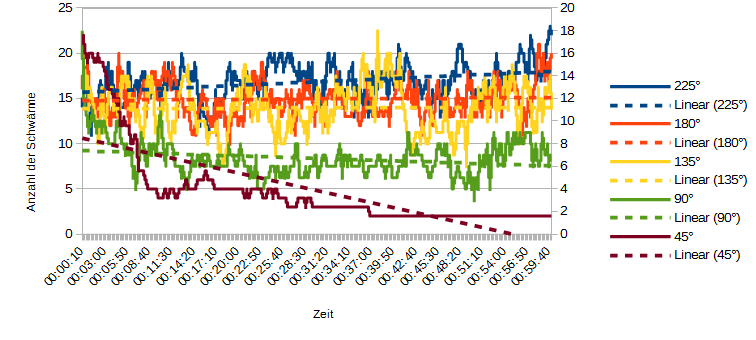
\includegraphics[width=\textwidth,height=\statisticHeight]{graphics/Statistics/FlockGeneral/LocalRange1Speed01ToFlock0.png}
	\caption{Entwicklung der Schwärme in Abhängigkeit ihres freien Willens}
	\label{pic:GeneralFlockStatistic1}
\end{figure}

Zu sehen ist, dass der Schwarm bei einem freien Willen von 90° und weniger dazu neigt sich zu gruppieren. Der Drang sich nach seinen Nachbarn auszurichten und in die selbe Richtung wie diese zu fahren, ist deutlich größer als der freie Wille der sie auseinander bringen würde. Auf lange Sicht wäre die Zahl der Schwärme Richtung 1 gesunken, da sich die Roboter immer weiter zusammengeballt haben. Dies ist vor allem bei 45° freiem Willen zu sehen, da die Schwärme, im Gegensatz zu 90°, kaum noch aufbrechen und relativ stabil bleiben. Während einigen der einstündigen Stimulationen trat dieser Fall sogar ein. Will man seine Roboter zusammenballen, ist es also sinnvoll den freien Willen geringer zu halten.

Bei 180° und 135° freiem Willen ist die Grenze, an der die Schwärme von Anfang bis Ende nahezu konstant bleiben. Sie brechen genauso schnell auseinander wie sie zusammen kommen, wodurch sich am Gesamtzustand der Schwärme wenig verändert. Dieser Breich ist damit gut geeignet um den Schwarm neutral zu lassen und weder zusammenballen zu lassen, noch zu verstreuen.

Ab einem freien Willen von 225° (112.5° in beide Richtungen) zeigt sich, dass die Roboter eher dazu neigen sich zu verteilen statt sich zu sammeln. Der Einfluss der Regel, sich wie seine Nachbarn auszurichten, macht weniger als 50\per bei der Berechnung des endgültigen Winkels aus und hat gegenüber dem freien Willen somit das Nachsehen.

\paragraph*{Warum haben sich trotzdem Schwärme gebildet?}
Einerseits resultiert es daraus, dass aus der Menge [-112.5°, 112.5°] der letztliche Wert zufällig ermittelt wurde, der Durchschnitt also um 0° herum liegt, mit einer durchschnittlichen Abweichung von 56.25° zu beiden Seiten.
Anderseits spielt aber auch der mangelnde Platz zum verteilen eine Rolle. Roboter die zufällig in die lokale Reichweite anderer Roboter gefahren sind, werden im nächsten Tick als Schwarm erkannt, unabhängig vom Grund warum sie zusammen waren.

\subsection*{Statistik: Gruppendrang}

\begin{table}[h]
	\caption{Eigenschaften des Schwarms}
	\begin{tabular}{ll}
		Größe des Schwarms:		& 25 Roboter \\
		Lokale Reichweite:		& 5\per der Größe der Simulation \\
		Geschwindigkeit:		& 10\per der lokalen Reichweite \\
		Drang zur Gruppierung:	& Variabel \\
		Freier Wille:			& 90° bzw 225° \\
	\end{tabular}
\end{table}

In~\autoref{pic:GeneralFlockStatistic2} und~\autoref{pic:GeneralFlockStatistic3} zu sehen, sind Statistiken die die Entwicklung von Schwärmen mit verändertem Drang zur Gruppierung zeigen. Über die X-Achse hinweg ist die Zeit der Simulation von 0-60 Minuten, die Y-Achse zeigt die Anzahl der vorhandenen Schwärme. In der ersten Statistik behielten sie dabei einen freien Willen von 90°, bei der zweiten wurde ein freier Wille von 225° eingestellt.

\subsubsection*{Freier Wille: 90°}

\begin{figure}[h]
	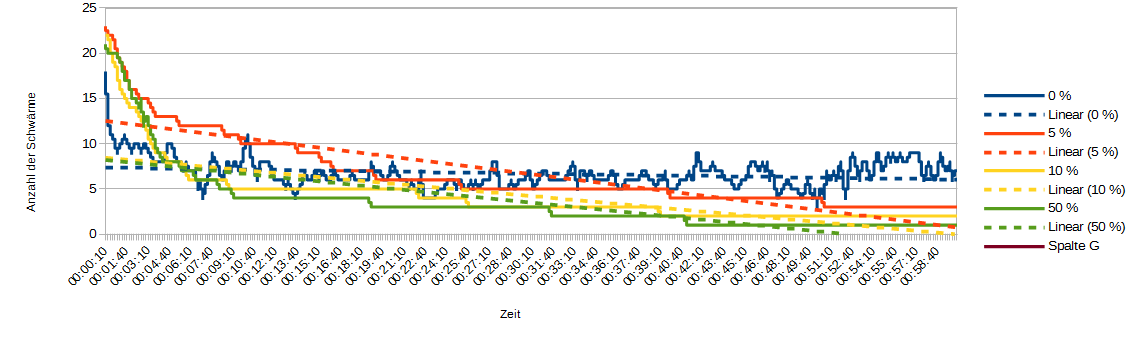
\includegraphics[width=\textwidth, height=\statisticHeight]{graphics/Statistics/FlockGeneral/LocalRange1Speed01FreeWill90.png}
	\caption{Entwicklung der Schwärme in Abhängigkeit ihres Dranges zur Gruppierung mit 90° eigenem Willen}
	\label{pic:GeneralFlockStatistic2}
\end{figure}

Bei einem freien Willen von 90° ist zu sehen, dass die Anzahl der Schwärme bei einem Drang zur Gruppierung von 0\per konstant bleibt. Diese Entwicklung war bereits in \autoref{subsubsec:StatistikFreierWille} zu sehen. Die Start-Anzahl war dabei in allen Simulationen annähern gleich.
Sobald der Drang zur Gruppierung über 0\per steigt, zeigt sich, dass die Roboter sich abhängig vom eingestellten Wert unterschiedlich schnell zu Schwärmen zusammenziehen und diese auch nicht wieder verlassen. Ein höherer Wert sorgte dabei analog dafür, dass sich die Schwärme schneller sammelten. Dennoch arbeitet der Wert des Gruppendrangs prozentual. Die Berechnung findet auf der Spanne von [Schwarm-Mittelpunkt, vorige Ausrichtung] statt. Entsprechend hat der freie Wille noch immer einen großen Einfluss auf die Schwärme, wenn sie auch durch den Gruppendrang jetzt stabiler sind.

\subsubsection*{Freier Wille: 225°}

Bei einem freien Willen von 225° zeigt sich dagegen deutlich mehr Varianz. Die Entwicklung um 0\per herum ist dabei wieder die gleiche wie in \autoref{subsubsec:StatistikFreierWille} bereits zu sehen war. Ein Wert von 5\per neigt die Trendlinie zwar leicht nach unten, die Daten zeigen aber nach wie vor hohe Fluktuationen und Schwärme die sich zunächst gebildet haben, brechen aufgrund des großen freien Willens wieder auseinander und die Roboter trennen sich. Bei 10\per wird der Trend zur Gruppierung zwar umso deutlicher, die Fluktuationen sind aber nach wie vor gut zu sehen und die Schwärme neigen noch immer dazu sich gelegentlich zu trennen. Erst ab einem Wert von 50\per bleiben die Schwärme immer stabil und langsam aber sicher fügen sich alle Roboter zu einem einzelnen Schwarm zusammen.

\begin{figure}[h]
	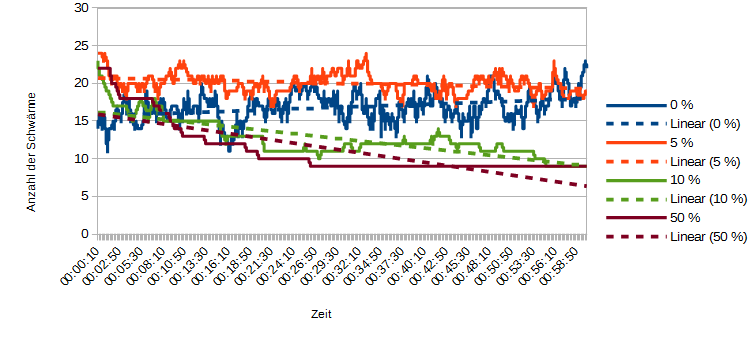
\includegraphics[width=\textwidth, height=\statisticHeight]{graphics/Statistics/FlockGeneral/LocalRange1Speed01FreeWill225.png}
	\caption{Entwicklung der Schwärme in Abhängigkeit ihres Dranges zur Gruppierung mit 225° eigenem Willen}
	\label{pic:GeneralFlockStatistic3}
\end{figure}

Allgemein lässt sich also sagen, dass der freie Wille einen großen Einfluss darauf hat, wie schnell sich die Schwärme zusammenfinden, wohingegen der Gruppendrang seinen Teil dazu beiträgt, die Schwärme stabil zu halten. Dies kommt eben auch daher, dass der Gruppendrang auf dem freien Willen aufsetzt. Ein höherer freier Wille macht auch den Gruppendrang 'stärker'.

\subsection*{Statistik: Negativer Gruppendrang}

Zum Schluss wurde noch eine Statistik mit negativen Gruppendrang erstellt. Hintergrund dieses Versuchs war es, die Roboter verteilen zu lassen. Damit sie sich während des Leerlaufs nicht versammeln und so in ihrer Masse zu einem größeren Hinderniss werden, wurde versucht die Roboter dazu zu bringen sich zu meiden und damit auszulösen, dass sie sich verteilen.
Der Wert des freien Willens von 45° wurde absichtlich so gering gewählt, dass dieser normalerweise dafür sorgt, dass die Schwärme sich schnell bündeln. Außerdem baut der Gruppendrang auf dem freien Willen auf, ein kleinerer freier Wille sollte den Effekt des Gruppendrangs dementsprechend auch gering halten.

\begin{table}[h]
	\caption{Eigenschaften des Schwarms}
	\begin{tabular}{ll}
		Größe des Schwarms:		& 25 Roboter \\
		Lokale Reichweite:		& 5\per der Größe der Simulation \\
		Geschwindigkeit:		& 10\per der lokalen Reichweite \\
		Drang zur Gruppierung:	& Variabel \\
		Freier Wille:			& 45° \\
	\end{tabular}
\end{table}

Über die X-Achse von \autoref{pic:NegativerGruppendrang} hinweg ist die Zeit der Simulation von 0-60 Minuten, die Y-Achse zeigt die Anzahl der vorhandenen Schwärme.
Wie zu sehen ist, versuchen sich die Roboter bei einem  freien Willen von 45° und einem Gruppendrang von 0\per zu Schwärmen zusammenzuschließen.
Dieses Verhalten ist nachvollziehbar, da ein derart geringer freier Wille dazu führt, dass die Bewegung größenteils davon abhängig ist die anderen zu imitieren. Roboter im Radius ihrer lokalen Reichweite fahren also meist in die selbe Richtung und gruppieren sich so auf natürliche Weise. Wenn sie gegen die Grenzen der Simulation stoßen und versuchen dieser auszuweichen, kommen sie dabei noch näher zusammen.

\begin{figure}[h]
	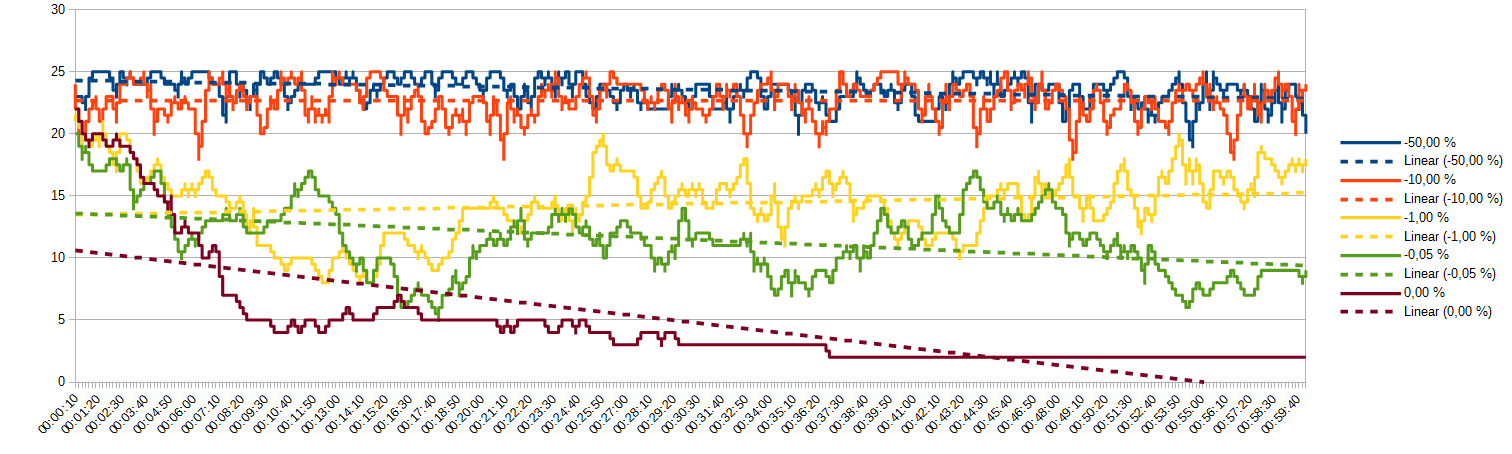
\includegraphics[width=\textwidth, height=\statisticHeight]{graphics/Statistics/FlockGeneral/LocalRange1Speed01FreeWill45NegativeToFlock.png}
	\caption{Entwicklung der Schwärme mit negativem Gruppendrang}
	\label{pic:NegativerGruppendrang}
\end{figure}

Ein negativer Gruppendrang von bereits 0.05\per reicht jedoch aus um die Trendlinie merklich nach oben zu verlagern und die Gruppierung in Schwärmen zumindest langsamer vollziehen zu lassen. Die Fluktuationen nehmen deutlich zu und die Schwärme scheinen nun deutlich instabiler zu sein. Zwar finden sich immer wieder Roboter in Schwärmen ein, sie brechen aber auch oft auseinander und die Einheiten gehen wieder getrennte Wege.

Auch hier lässt wieder deutlich sehen, dass der freie Wille der ausschlaggebende Wert ist, wenn es darauf ankommt die Roboter zusammenzuführen, wohingegen der der Gruppendrang dafür sorgt, dass die Schwärme in sich stabil bleiben und die Roboter nicht versuchen abzudriften.

Schon ab 1\per negativen Gruppendrangs zeigt die Trendlinie, dass die Gruppen eher dazu neigen sich aufzulösen statt sich neu zu bilden. Der Winkel zur Mitte des eigenen Schwarms kann maximal 180° (in beide Richtungen) groß sein, das heißt der negative freie Wille kann einen Einfluss von maximal 1.8° einnehmen. Trotzdem reicht bereits dieser Einfluss aus um die Roboter dazu zu bewegen sich voneinander zu entfernen.

Ab einem Wert von 10\per zeigt sich letztlich eine totale Streuung und die Trendlinie bleibt eine Konstante. Die Roboter schaffen es teilweise keinen einzigen Schwarm zu bilden (bzw. nur Schwärme in denen sie selbst als einziger Roboter vertreten sind).

Überraschenderweise zeigt ab einem Wert von 50\per die Trendlinie wieder nach unten und die Roboter scheinen sich erneut zu gruppieren. Der Grund hierführ ist, dass die Roboter beim Ausweichen ihrer Kollegen überschießen und sich so weit in die andere Richtung drehen, dass sie letztlich vom Winkel wieder näher dran sind als vorher. Legt man Wert darauf, dass sich die Roboter verteilen, gilt es also einen passenden Prozentwert einzustellen und diesen nicht zu übertreiben, da man sonst das Gegenteil dessen erreicht, was man als Ziel hatte.







\section{Anführer}

\newcommand{\sectionLeaderPictureStats}{width=7.5cm, height=4cm}

Nachdem der Anführer implementiert wurde, wurde das konzipierte Verhalten getestet und verschiedene Statistiken erhoben, inwiefern ein Anführer in der Lage ist einen Schwarm an sein Ziel zu führen, ohne dass diese aktiv gesteuert werden müssen.
Dafür wurde der gesamte Schwarm an einer Ecke der Simulation platziert. Die Einheiten waren dabei immer nahe genug beieinander, um als einzelner Schwarm angesehen zu werden, aber ansonsten zufällig verteilt. Einem der Roboter wurde daraufhin zufällig eine \highlight{New\_Mission} zugeteilt und damit zum Anführer gewählt. Dieser hat daraufhin versucht seinen Schwarm zum Ziel zu führen.

Auch in dieser Analyse spielt der Zufall eine beachtliche Rolle, da der freie Wille der Einheiten darauf ausgelegt ist. Es wurden daher immer 15 Simulationen durchgeführt und aus den mittleren 9 Ergebnissen ein Mittelwert berechnet, um Aureißer möglichst zu ignorieren.

\subsection*{Nachbesserung der Implementierung}\label{subsec:AnalyseNachbesserung}

\begin{wrapfigure}{r}{\pictureWidthSmall}
	\includegraphics[width=\pictureWidthSmall,keepaspectratio]{graphics/AlgorithmusAnführerFixed.png}
	\caption{Entfernungen des Anführers}
	\label{pic:AnführerReichweitenFixed}
\end{wrapfigure}

Recht schnell hat sich gezeigt, dass das Einfangen des Schwarms, wie es in \autoref{subsubsec:AnführerEinfangen} vorgestellt wurde, mehr negative als positive Auswirkungen hat. Versuchte der Roboter seinen Schwarm einzufangen, änderte er, dadurch dass er sich um 180° umdrehen musste, die gesamte Ausrichtung des Schwarms. Dies führte in den Simulationen meist dazu, dass der Schwarm vollkommen abgedriftet ist und der Anführer Mühe und Not hatte, ihn wieder auf das Ziel auszurichten. Meist verlor er dabei den Schwarm wieder, noch bevor dieser wieder ausgerichtet war, womit das Manöver wieder von vorne los ging. Durch dieses Fehlverhalten mussten die meisten Simulationen abgebrochen werden und die Ergebnisse waren letztlich unbrauchbar, da zu viel von Hand gefiltert werden musste.

Aus diesem Grund wurde der Teil des Algorithmus' wieder entfernt. Stattdessen wartet der Anführer nun, wenn der Schwarm 50\per der lokalen Reichweite entfernt ist und gibt auf, wenn der Schwarm-Mittelpunkt die eigene lokale Reichweite ganz verlassen hat. Aufgeben bedeutet in diesem Kontext, dass der Anführer ohne seinen Schwarm zum Ziel gefahren ist. Dies führte allgemein zu besseren Ergebnissen und der Schwarm konnte zumindest in Teilen zum Ziel gebracht werden.

\subsection*{Abhängigkeit: Freier Wille}\label{subsubsec:AbhängigkeitFreierWille}

\begin{table}[h]
	\caption{Eigenschaften des Schwarms}
	\begin{tabular}{ll}
		Größe des Schwarms:		& 25 Roboter \\
		Antahl Anführer:		& 1 \\
		Lokale Reichweite:		& 5\per der Größe der Simulation \\
		Geschwindigkeit:		& 10\per der lokalen Reichweite \\
		Drang zur Gruppierung:	& 5\per \\
		Freier Wille:			& Variabel \\
	\end{tabular}
\end{table}

In dieser Simulation wurde geprüft, wie sich verschiedene Werte für den freien Willen darauf auswirken, dass der Schwarm zum Ziel geführt werden kann. Über die X-Achse von \autoref{pic:LeaderDependencyFreeWill} hinweg ist die vergangene Wegstrecke in Prozent angegeben, die Y-Achse zeigt die Anzahl der Roboter die im Schwarm des Anführers vorhanden sind.
In der Statistik zu sehen, ist dass der Schwarm anfangs immer zusammen blieb. Da die Roboter als gemeinsamer Schwarm zusammen gestartet sind, mussten sie sich nicht erst finden. Außerdem musste der Anführer erst einmal eine gewisse Zeit lang fahren, bevor der anfängliche Schwarm nicht mehr als sein Schwarm registriert wird.

\begin{figure}[h]
	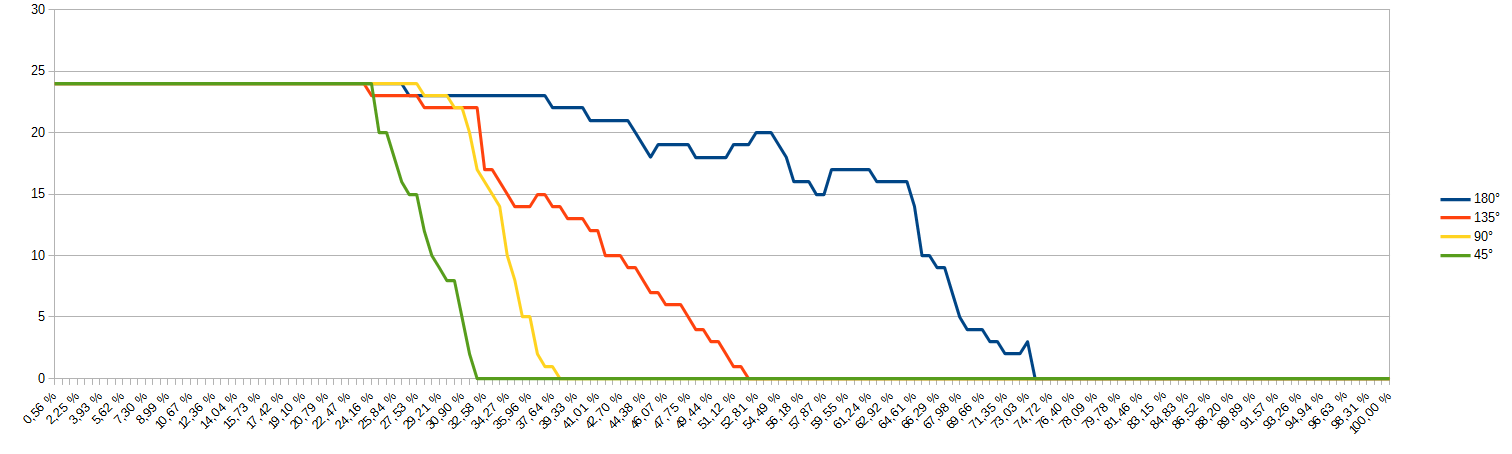
\includegraphics[width=\textwidth, height=\statisticHeight]{graphics/Statistics/Leader/DependencyFreeWill.png}
	\caption{Erfolg eines Anführer ins Abhängigkeit des freien Willens}
	\label{pic:LeaderDependencyFreeWill}
\end{figure}

Wenn der Schwarm in eine andere Richtung lenkte als der Anführer, blieb der Anführer ab 50\per seiner lokalen Reichweite stehen und wartete. Zog der Schwarm weiterhin in eine verkehrte Richtung, löste er sich irgendwann vom Anführer und dieser zog alleine weiter Richtung Ziel. Durch den relativ hohen Wert von 5\per im Gruppendrang blieb der Schwarm immer gut zusammen. Bei geringeren werten des freien Willens zog er öfter im gesamten davon, während die Roboter bei mehr freiem Willen immer mehr Stück für Stück weg zogen.

Je niedriger der Wert im freien Willen war, desto eher löste sich der Schwarm scheinbar von seinem Anführer. Dies ist darauf zurückzufiühren, dass bei einer Gruppengröße von 25 Robotern der Einfluss eines Anführers nur 4.2\per ausmacht und der Schwarm mehr vom Zufall als vom Anführer gelenkt wird. Dass die Roboter mit dem größeren freien Willen letztlich scheinbar länger beim Anführer blieben, ist dem geschuldet, dass die Roboter weniger eng als Schwarm zusammen bleiben und durch die Verteilung der Roboter mehr in der Nähe des Anführers blieben. Die Roboter mit dem geringen freien Willen hingegen blieben mehr zusammen und sind somit als ganzes abhanden gekommen.

\subsection*{Abhängigkeit: Gruppengröße und -drang}

\begin{table}[h]
	\caption{Eigenschaften des Schwarms}
	\begin{tabular}{ll}
		Größe des Schwarms:		& Variabel \\
		Anzahl Anführer:		& 1 \\
		Lokale Reichweite:		& 5\per der Größe der Simulation \\
		Geschwindigkeit:		& 10\per der lokalen Reichweite \\
		Drang zur Gruppierung:	& Variabel \\
		Freier Wille:			& 90° \\
	\end{tabular}
\end{table}

In den folgenden Statistiken wurde ein Anführer mit steigender Gruppenzahl und unterschiedlichem Gruppendrang gemessen. Über die X-Achse von \autoref{pic:LeaderDependencyFreeWill} hinweg ist der eingestellte Gruppendrang angegeben.
Das erste Diagramm zeigt dabei, für wie viel Prozent der Wegstrecke der Anführer erfolgreich war. Erfolgreich war er, wenn der gesamte Schwarm bei ihm blieb. Ging auch nur ein Roboter abhanden, war der Anführer ab dort nicht mehr erfolgreich.
Das zweite Diagramm zeigt die Größe des Schwarms um den Anführer herum beim erreichen des Ziels. Wenn der Anführer nicht alle Roboter beisammen hielt, ist es dennoch interessant zu wissen, wie viele Roboter es im Durchschnitt mit ihm zum Ziel geschafft haben.
Das dritte Diagramm zeigt die Anzahl der Wartezeiten die der Anführer hatte. Eine höhere Anzahl an Wartezeiten ist direkt equivalent zu einer längeren Zeit die die Simulation gebraucht hat.

Dabei werden immer 2 Werte gezeigt. 'Mittelwert', der einen einfachen Mittelwert über alle 15 Messwerte anzeigt und 'Median', bei dem der Mittelwert auf die mittleren 11 Messwerte begrenzt wurde um Ausreißer auszusortieren. Da der Anführer selbst immer am Ziel ankommt, wurde er bei den Messwerten abgezogen. Die Anzahl der dargestellten Roboter entspricht also immer denjenigen, die passiv zum Ziel geführt wurden.

\subsubsection*{5 passive Roboter}


In \autoref{pic:LeaderSize5} zu sehen ist zunächst einmal, dass der Anführer in einer Gruppe mit nur 5 Robotern einen sehr starken Einfluss auf die Gruppe hat. Bereits ohne Gruppendrang gibt es eine Erfolgsquote von über 20\%. Ab 5\per Gruppendrang gibt es schon annähernd 80\per Erfolgsquote und ab 10\per bekommt der Anführer seinen Schwarm immer vollständig ans Ziel gebracht. Median und Mittelwert sind meist relativ nahe zusammen, was bedeutet dass es sehr wenige Ausreißer gab, wenn überhaupt.

Die Größe des Schwarms zeigt ein sehr ähnliches Bild. Kommen bei 0\per Gruppendrang im Schnitt nur sehr wenige Roboter an, steigert es sich sprunghaft auf 4 Einheiten und ab einem Gruppendrang von 10\per kommen immer alle Roboter an. Trotz einem Einfluss von 16.6\per kann sich der Anführer also nicht durchsetzen, wenn es keinen Gruppendrang gibt.

\begin{figure}[h]
	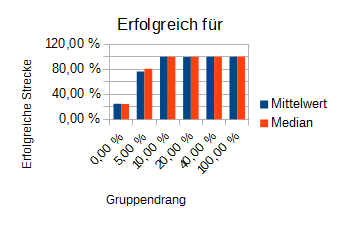
\includegraphics[\sectionLeaderPictureStats]{graphics/Statistics/Leader/FlockSize/5_1.png}
	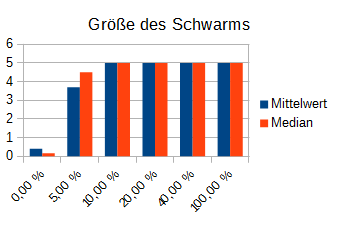
\includegraphics[\sectionLeaderPictureStats]{graphics/Statistics/Leader/FlockSize/5_2.png}
	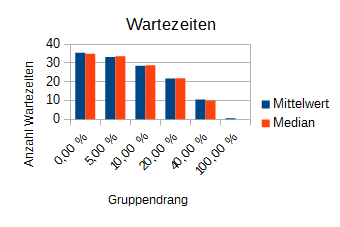
\includegraphics[\sectionLeaderPictureStats]{graphics/Statistics/Leader/FlockSize/5_3.png}
	\caption{Erfolg eines Anführer ins Abhängigkeit der Gruppengröße und des Gruppendrangs mit 5 passiven Robotern}
	\label{pic:LeaderSize5}
\end{figure}

Die Wartezeiten sind nicht ganz so konstant, zeigen aber, dass es noch deutliche Unterschiede zwischen den Prozentwerten im Bereich von 10-100\per gibt, auch wenn die beiden vorigen Diagramme dort keine mehr gezeigt haben. Mit einem höheren Gruppendrang sinkt die Anzahl der Wartezeiten immer mehr und bei 100\per gibt es sogar annähernd gar keine mehr.

Bei 100\per Gruppendrang zeigt sich generell überall das beste Ergebnis, was nicht weiter verwunderlich ist. Bei 100\per richten sich die Roboter alle ausschließlich nach ihrer Mitte aus. Diese Konfiguration gab es nur in dieser ersten Statistik. Sie dürfte für die anderen nicht anders ausfallen und zeigen eher, dass das Konzept in dieser Hinsicht generell funktioniert. Eine Abweichung von einem perfekten Ergebnis (abgesehen bei den Wartezeiten) hätte höchstwahrscheinlich auf einen Fehler in der Implementierung hingewiesen.

\newpage
\subsubsection*{10 passive Roboter}

Die Diagramme in \autoref{pic:LeaderSize10} zeigen, dass der Einfluss des Anführers mit 5 Robotern mehr schon deutlich nachlässt. Konnten vorher schon ab 10\per Gruppendrang beste Ergebnisse erziehlt werden, zeigt der Durchschnitt nun deutlich niedrigere Werte. Außerdem liegen der Mittelwert und der Median nicht mehr so eng beieinander. Dies bedeutet vor allem, dass die Fehlerquote zunahm und die 11 mittleren Ergebnisse nun ebenfalls höhere Schwankungen aufweisen. Nur bei 40\per sieht man noch einen vollen Erfolg über alle Messwerte hinweg.

\begin{figure}[h]
	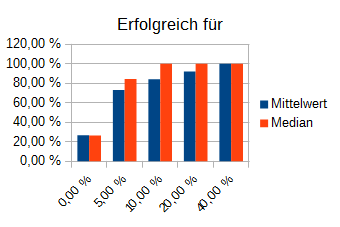
\includegraphics[width=7.5cm, keepaspectratio]{graphics/Statistics/Leader/FlockSize/10_1.png}
	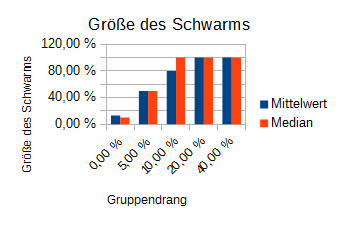
\includegraphics[width=7.5cm, keepaspectratio]{graphics/Statistics/Leader/FlockSize/10_2.png}
	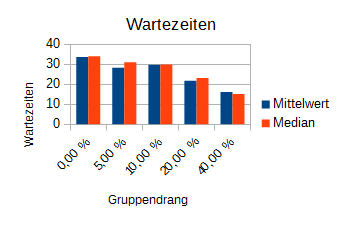
\includegraphics[width=7.5cm, keepaspectratio]{graphics/Statistics/Leader/FlockSize/10_3.png}
	\caption{Erfolg eines Anführer ins Abhängigkeit der Gruppengröße und des Gruppendrangs mit 10 passiven Robotern}
	\label{pic:LeaderSize10}
\end{figure}

Die Größe des Schwarms ist von ähnlichen Rückschlägen betroffen. Bei 0\per Gruppendrang schafft es nur jeder zehnte Roboter ins Ziel, fast der gleiche Wert wie bei 5 passiven Robotern. Bei 5\per Gruppendrang ist die Erfolgsquote jedoch von 90\per auf 50\per gesunken (bezogen auf den Median).
Bei 10\per Gruppendrang schafft es der Median noch auf einen vollen Erfolg, der Mittelwert hingegen, der in \autoref{pic:LeaderSize5} noch bei 100\per stand, ist nun auf 80\per gesunken.

Die Wartezeiten hingegen zeigen nicht unbedingt den gleichen Trend, wenn auch hier Mittelwert und Median weiter auseinander sind als beim Vorgänger \autoref{pic:LeaderSize5}. Sie sind zwar allgemein gestiegen, was zu erwarten war, wenn der Platz aufgrund weniger Roboter nun knapper wird. Der Trend ist aber nicht mehr so steil wie zuvor. Steigen beide Diagramme bei ca. 35 Wartezeiten ein, ist der Trend nun flacher und bei 40\per Gruppendrang nun eine deutlich höhere Wartezeit zu sehen (+50\%).

\newpage
\subsubsection*{15 passive Roboter}

\begin{figure}[h]
	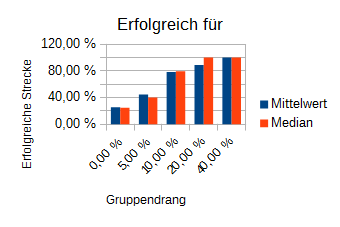
\includegraphics[width=7.5cm, keepaspectratio]{graphics/Statistics/Leader/FlockSize/15_1.png}
	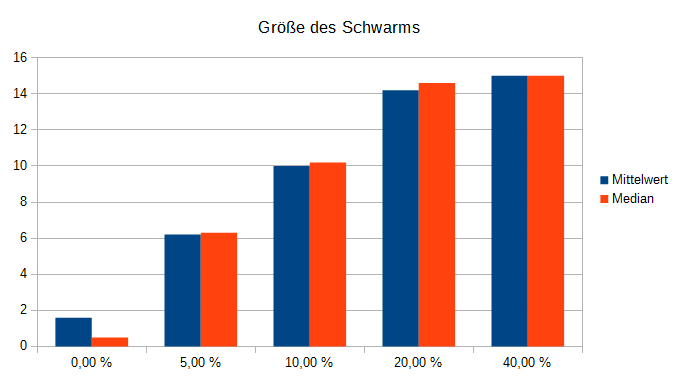
\includegraphics[width=7.5cm, keepaspectratio]{graphics/Statistics/Leader/FlockSize/15_2.png}
	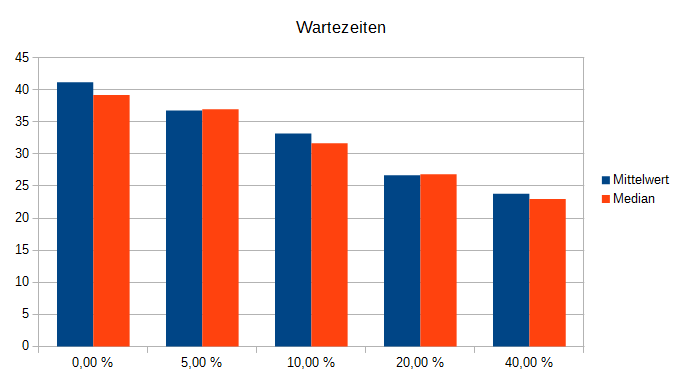
\includegraphics[width=7.5cm, keepaspectratio]{graphics/Statistics/Leader/FlockSize/15_3.png}
	\caption{Erfolg eines Anführer ins Abhängigkeit der Gruppengröße und des Gruppendrangs mit 15 passiven Robotern}
	\label{pic:LeaderSize15}
\end{figure}

In \autoref{pic:LeaderSize15} nimmt der allgemeine Trend weiter seinen Lauf. Die Erfolgsquote für die Werte unter 40\per nehmen immer weiter ab, wenn auch die 40\per selbst noch einen vollen Erfolg vorweisen kann.

Es kommen auch weniger Roboter insgesamt im Ziel an, wenn die Gesamtzahl der ankommenden Roboter auch bei 20\per Gruppendrang noch recht hoch ist. Bei 40\per Gruppendrang ist nach wie vor ein voller Ausschlag zu sehen.

Auch die Wartezeiten zeigen den selben Trend wie zuvor. Sie starten recht hoch, der Trend bleibt aber flacher als bei den Messungen mit 5 passiven Robotern weniger.

\subsubsection*{20 passive Roboter}

\begin{figure}[h]
	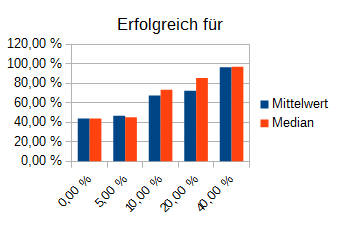
\includegraphics[width=7.5cm, keepaspectratio]{graphics/Statistics/Leader/FlockSize/20_1.png}
	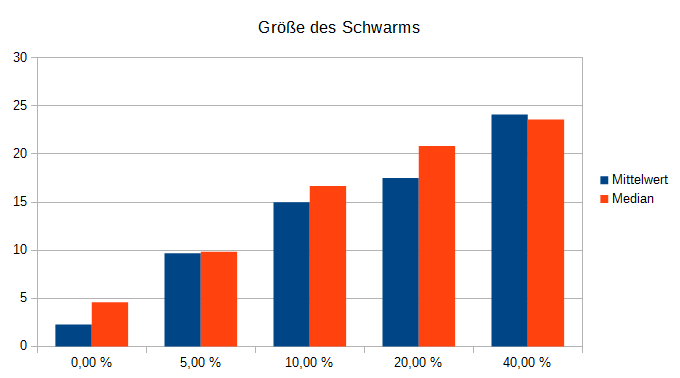
\includegraphics[width=7.5cm, keepaspectratio]{graphics/Statistics/Leader/FlockSize/20_2.png}
	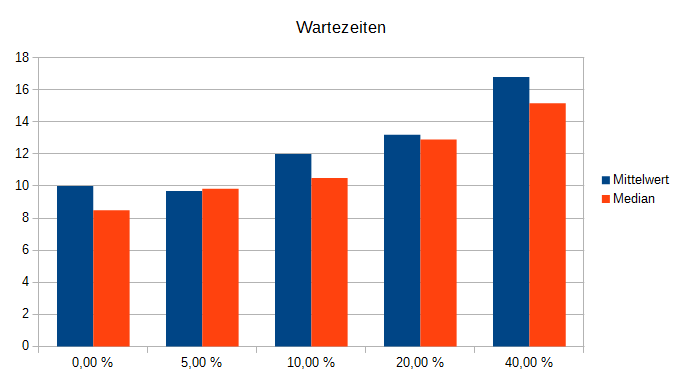
\includegraphics[width=7.5cm, keepaspectratio]{graphics/Statistics/Leader/FlockSize/20_3.png}
	\caption{Erfolg eines Anführer ins Abhängigkeit der Gruppengröße und des Gruppendrangs mit 20 passiven Robotern}
	\label{pic:LeaderSize20}
\end{figure}

Ab einer passiven Anzahl von 20 Robotern zeigt sich in \autoref{pic:LeaderSize20} erstmals der Trend, dass die Wartezeiten zunehmen, wenn der Gruppendrang größer wird. Ein genauerer Blick auf das Diagram zeigt jedoch auch, dass die Wartezeiten allgemein sehr viel niedriger sind als in den Messungen mit weniger Robotern.

Dies ist vor allem darauf zurückzuführen, dass der Anfüher ab einer Zahl von 20 passiven Robotern einen Schwarm viel schneller vollständig verliert und es keine Wartezeiten mehr gibt, weil er schneller dazu übergeht das Ziel alleine aufzusuchen. Auch die anderen beiden Diagramme zeigen nun bei 40\per Gruppendrang keinen vollen Erfolg mehr.

\subsubsection*{25 passive Roboter}

\begin{figure}[h]
	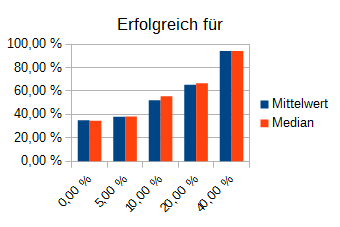
\includegraphics[width=7.5cm, height=4cm]{graphics/Statistics/Leader/FlockSize/25_1.png}
	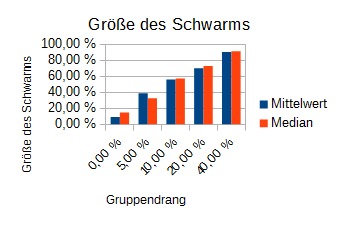
\includegraphics[width=7.5cm, height=4cm]{graphics/Statistics/Leader/FlockSize/25_2.png}
	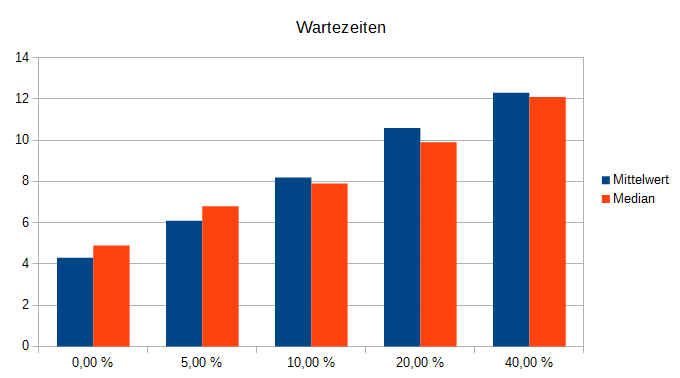
\includegraphics[width=7.5cm, height=4cm]{graphics/Statistics/Leader/FlockSize/25_3.png}
	\caption{Erfolg eines Anführer ins Abhängigkeit der Gruppengröße und des Gruppendrangs mit 25 passiven Robotern}
	\label{pic:LeaderSize25}
\end{figure}

In den letzten Diagrammen (\autoref{pic:LeaderSize25}) ist letztlich zu sehen dass sich der allgemeine Trend weiter fort führt. Die Wartezeiten sinken noch deutlicher, weil der Anführer seinen Schwarm immer früher verliert. Die erfolgreiche Strecke nimmt genau wie die Anzahl der Roboter die im Ziel ankommen immer mehr ab. Nur bei 40\per Gruppendrang bleiben die Werte noch immer recht hoch.











\section{Transport von Waren mit Hilfe eines Schwarms}\label{sec:EvaluationTransport}

Nun da alles zusammengesetzt ist, gilt es letzte Messungen zu machen und zu schauen, wie sich die Roboter unter verschiedenen Bedingungen beim Transport machen.

Bei den folgenden Statistiken wurden jeweils 15 Simulationen durchgeführt und die mittleren 11 zu einem Durchschnitt verrechnet um Ausreißer zu eliminieren. Die Roboter wurden zufällig auf der gesamten Simulation erstellt und nach wenigen Sekunden der Auftrag gesendet. Sobald sie alle versammelt waren, wurde die Aufzeichnung gestartet und der Schwarm machte sich auf den Weg zum Ziel. Dabei wurden 4 verschiedene Eigenschaften beobachtet:

\paragraph*{Observations}
Dies ist die Anzahl der Ticks die während des Transports verstrichen sind. Da ein Tick genau 1.1s dauert, ist es damit auch ein direktes Equivalent für die Zeit die der Transport gedauert hat.

\paragraph*{LengthOfSlack}
Von einem Tick zum anderen wurde gemessen, wie viel sich die einzelnen Roboter in Relation zur Mitte des Objektes bewegt haben. Dadurch wurde der Schlupf berechnet, den es während des Transports gab. Zu bedenken ist bei diesem Wert allerdings, dass die Simulation über keine Berechnung von Reibung verfügt, die Roboter also eine unendliche Kraft besitzen. Die Werte stellen demnach eine obere Grenze dar, für den Schlupf der in der Realität entstehen könnte.

\paragraph*{LengthOfDrivenWay}
Verdeutlicht den Weg, der von einem Roboter durchschnittlich zurückgelegt wurde. Die direkte Strecke vom Start zum Ende hat eine Länge von 5.656 (ROS-Einheiten). Da das Transportobjekt nur innerhalb der Reichweite von 0.05 am Ziel sein musste, ergibt sich somit eine Strecke von 5.606 Einheiten die gefahren werden musste.

\paragraph*{LeaderDidntMove}
Letztlich wurde noch gemessen, wie oft es vor kam, dass ein Anführer sich nicht bewegen konnte, weil ein anderer Roboter ihm den Weg versperrte.

\subsection*{Abhängigkeit: Größe des Flocks und Anzahl Anführer}

In den ersten Simulationen wurden verschiedene Kombinationen von passiven Robotern und Anführern getestet.

Unschwer zu sehen ist, dass der Transport mit 5 Robotern und 1 Anführer am längsten dauert, mit 66 Ticks. Überraschend jedoch ist, dass 10 Roboter und 2 Anführer schneller ist und 15 Roboter mit 3 Anführern wieder etwas schneller. Die Geschwindigkeit ist also nicht unbedingt nur davon abhängig, wie viel Prozent der Roboter Anführer sind. Generell ist der Transport schneller, je mehr Roboter man hat.

\begin{figure}[h]
	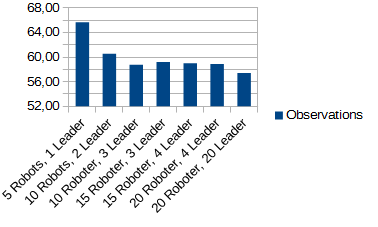
\includegraphics[width=7.5cm,keepaspectratio]{graphics/Statistics/Transport/Number_Observations.png}
	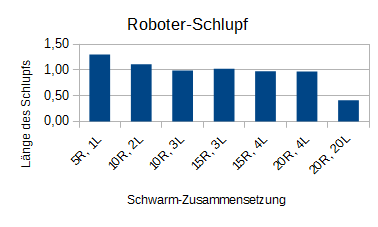
\includegraphics[width=7.5cm,keepaspectratio]{graphics/Statistics/Transport/Number_Slack.png}
	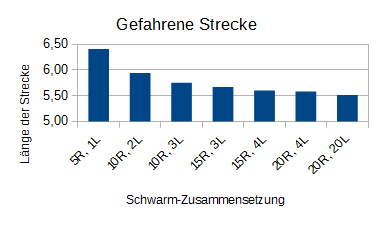
\includegraphics[width=7.5cm,keepaspectratio]{graphics/Statistics/Transport/Number_Way.png}
	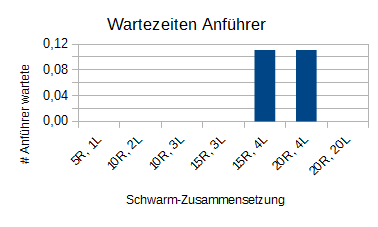
\includegraphics[width=7.5cm,keepaspectratio]{graphics/Statistics/Transport/Number_Move.png}
	\caption{Abhängigkeit: Größes des Flocks und Anzahl der Anführer}
	\label{pic:TransportNumber}
\end{figure}

Gestützt wird die Grafik von der Länge des Schlupfs, die ebenfalls abnimmt, wenn mehr Roboter den Auftrag erledigen, genau wie die Länge des Weges der pro Roboter gefahren wurde. Bei 20 Robotern und 4 Anführern, fuhren die Roboter (pro Roboter) 12.95\per weniger Strecke, als bei 5 Robotern mit 1 Anführer.
Im Schnitt hatten die Anführer keine Probleme sich zu bewegen. Nur in 2 Konfigurationen gab es überhaupt Ausschläge, diese bedeuten aber gerade mal einen Durchschnitt von 0.11 Stillständen.

Generell lässt sich also sagen, dass ein Auftrag tatsächlich schneller beendet werden kann, wenn er von mehr Robotern ausgeführt wird. Da er mit doppelt so vielen Robotern allerdings nicht doppelt so schnell ist, ist es letztlich wohl eine Abschätzung, ob die zusätzlichen Roboter besser einen eigenen Auftrag annehmen oder wirklich frei sind helfen können.

Der letzte Balken der Statistik zeigt den Transport mit allen Robotern als Anführer. Dies entspricht keinem Schwarm mehr, sondern streng gesteuerten Robotern und zeigt klar die Grenze, wie gut es generell werden kann. In jeder der 4 verschiedenen Eigenschaften stellen sie klar den besten Wert auf, wenn auch bei der Länge des Weges nur ganz knapp zum zweiten Platz.

\subsection*{Abhängigkeit: Freier Wille}

In der zweiten Runde von Simulationen wurde der freie Wille verändert. Bei 0° haben sich die Roboter streng nach ihren Nachbarn ausgerichtet und der einzige Zufall waren ihre Ausrichtungen bei Beginn des Transports. Entsprechend stellt diese Konfiguration wieder die Grenze auf, wie gut der Schwarm werden kann.

\begin{figure}[h]
	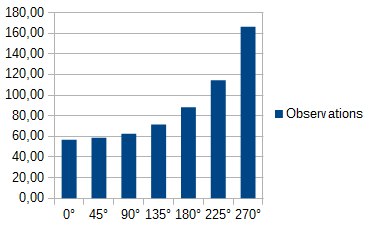
\includegraphics[width=7.5cm,keepaspectratio]{graphics/Statistics/Transport/Angle_Observations.png}
	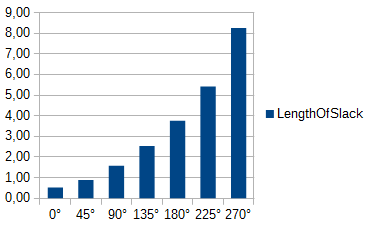
\includegraphics[width=7.5cm,keepaspectratio]{graphics/Statistics/Transport/Angle_Slack.png}
	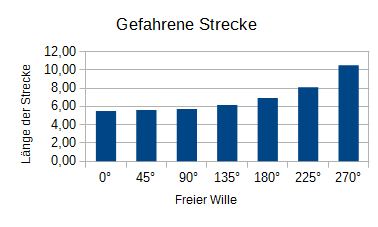
\includegraphics[width=7.5cm,keepaspectratio]{graphics/Statistics/Transport/Angle_Way.png}
	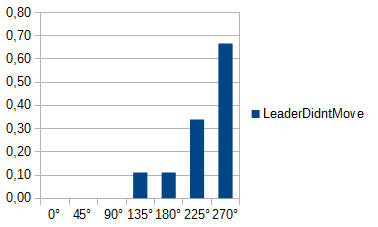
\includegraphics[width=7.5cm,keepaspectratio]{graphics/Statistics/Transport/Angle_Move.png}
	\caption{Abhängigkeit: Freier Wille}
	\label{pic:TransportAngle}
\end{figure}

Generell ist in dieser Runde, wenig überraschend zu sehen, dass der Transport besser wird, je geringer der freie Wille ist. Der Slack steigt bei einem freien Willen von 270° auf über 1600\per an. Ebenfalls haben die Anführer bis zu einem freien Willen von 90° keine Probleme sich zu bewegen. Erst ab da steigt der Balken deutlich an, ist aber immer noch recht gering, selbst bei 270°.

\subsection*{Abhängigkeit: Lokale Reichweite}

Die letzte Runde der Simulationen zeigt den Transport mit verschiedenen Reichweiten. Das Objekt ist 2x2 groß. Bei einer Reichweite von 4 ist das Transportobjekt von einer Ecke zur anderen abgedeckt. Bei einer lokalen Reichweite von 0.3 kommen sie gerade so über die eigene Größe hinaus, die 0.1 beträgt.

\begin{figure}[h]
	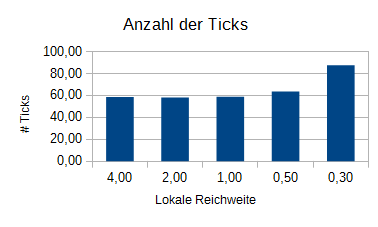
\includegraphics[width=7.5cm,keepaspectratio]{graphics/Statistics/Transport/Range_Observations.png}
	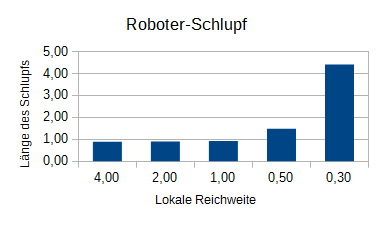
\includegraphics[width=7.5cm,keepaspectratio]{graphics/Statistics/Transport/Range_Slack.png}
	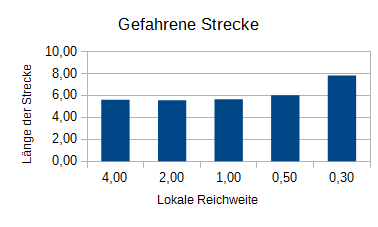
\includegraphics[width=7.5cm,keepaspectratio]{graphics/Statistics/Transport/Range_Way.png}
	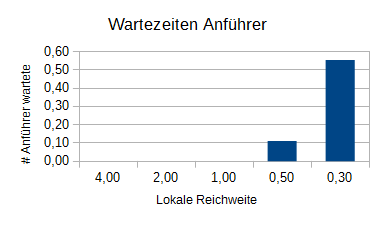
\includegraphics[width=7.5cm,keepaspectratio]{graphics/Statistics/Transport/Range_Move.png}
	\caption{Abhängigkeit: Lokale Reichweite}
	\label{pic:TransportRange}
\end{figure}

Bis zu einer lokalen Reichweite von 1 scheint dies aber keinen Effekt zu haben. Erst ab 0.5 zeigt sich ein kleiner Unterschied zu seinen Vorgängern, obwohl hier nur noch ein viel kleinerer Teil der Roboter innerhalb des Transportobjektes mit einbezogen werden konnte. Das bedeutet dass der Einfluss von Roboter über 1-2 Ecken hinweg nicht allzu viel abnimmt. Erst bei einer lokalen Reichweite von 0.3 wird der Fehlerbalken größer, ist aber immer noch recht gering, wenn man denkt, dass gerade einmal die eigene Größe Abstand zwischen den Robotern war.
